%Indice

%Premessa
%Cenni storici
%Descrizione Firewall Galliera
%Migrazione FW interno
%  Simulazione con lxc
%  Sistemi di automazione
%Il futuro
%  {\em iptables}
%  eBPF/XDP

\chapter{Introduzione} % Main chapter title

\label{Chapter1} % For referencing the chapter elsewhere, use \ref{Chapter1} 

%----------------------------------------------------------------------------------------

% Define some commands to keep the formatting separated from the content 
\newcommand{\keyword}[1]{\textbf{#1}}
\newcommand{\tabhead}[1]{\textbf{#1}}
\newcommand{\code}[1]{\texttt{#1}}
\newcommand{\file}[1]{\texttt{\bfseries#1}}
\newcommand{\option}[1]{\texttt{\itshape#1}}

%----------------------------------------------------------------------------------------

Il progetto di seguito presentato ha avuto origine da considerazioni
relative alla necessit\`a di aggiornare il sistema di firewall a protezione
della rete interna dell'ospedale Galliera.

La LAN dell'ospedale \`e connessa ad internet dal 1996 e sin da allora il
traffico di rete da e verso l'esterno \`e stato regolato e monitorato da
router/firewall Linux dei quali mi sono sempre occupato personalmente.

Nel tempo le esigenze di connettivit\`a sono via via aumentate ed i nostri
sistemi si sono dimostrati adeguati sia per quanto riguarda le funzionalit\`a
che per prestazioni.
Tuttavia nell'arco del 2017 si sono presentate alcune situazioni di
criticit\`a, causate sostanzialmente dal grande numero di regole sui firewall.

Pur avendo risolto i problemi, ho ritenuto di dover considerare questi segnali
di possibile obsolescenza del sistema, studiando le attuali alternative agli
strumenti scelti oramai circa 17 anni fa: cio\`e in pratica le alternative ad
iptables.  In effetti l'alternativa c'\`e: si chiama nftables ed nato proprio
con lo scopo di soppiantare iptables.

Il progetto, che si configura come studio di fattibilit\`a, \`e consistito
prima di tutto nell'approfondimento del nuovo framework. \`E seguita poi una
fase di riscrittura e di test delle regole dei due firewall in un ambiente
virtuale su scenari architettati ad-hoc. La sperimentazione \`e terminata e ha
fornito elementi utili per valutare l'opportunit\`a di mettere in atto la
migrazione. 


\chapter{Packet Filtering in Linux}

\label{Cenni storici} % For referencing the chapter elsewhere, use \ref{Chapter1} 

Per inquadrare l'argomento Linux firewall ritengo possa essere interessante
fornire un breve riassunto dell'evoluzione degli strumenti per la
classificazione ed il filtraggio dei pacchetti nel kernel Linux.

\section{Storia}
Nella tabella \ref{tab:history}
vengono considerati solo i rilasci nei kernel stabili. Fino alla serie 2.6.x le
nuove features venivano introdotte sperimentalmente nelle versioni con major
revision number dispari, ad esempio 2.3.4; a partire dalla versione 3 non
esiste più differenza tra kernel sperimentale e di produzione.
\begin{center}
  \label{tab:history}
  \begin{table}[ht]
    \centering % used for centering table
     \begin{tabular}{@{}lcccl@{}}
       \toprule
       {\bf Framework/tool} & {\bf Stateful} & {\bf Anno} & {\bf Kernel} & {\bf Coder}\\ \midrule
       ipfw     & no & 1994      & 1.0  & Alan Cox \\
       ipfwadm  & no & 1995-1999 & 1.2.$x$\marginnote{con $x>0$} - 2.0 & A. Cox e Jos Vos\\ [0.5ex]
       ipchains & no & 1999-2001 & 2.2  & Rusty Russell \\ [0.5ex]
       iptables & s\`i & 2001-     & 2.4  & Rusty Russell \\ [0.5ex]
       nftables & s\`i & 2014-     & 3.13 & gli stessi di iptables \\ [0.5ex]
       %eBPF/XDP & s\`i &       &      & \\ 
       \bottomrule
     \end{tabular}  
    \caption{Evoluzione dei framewrok (kernel versioni stabili)} % title of Table
  \end{table}
\end{center}
Le prime funzionalità di firewall sono state introdotte nel 1994 grazie al
lavoro di Alan Cox che ne ha fatto il porting dal codice di BSD Unix.
Questo codice costituisce la prima versione delle funzionalità di firewall
all'interno del kernel Linux. Il successore di ipfw è
stato ipfwadm, in realtà una riscrittura del corrispondente ipfw
di BSD da parte di Alan Cox e Jos Vos.
Ipfw e ipfwadm consentivano di realizzare le funzioni di base di un firewall:
\begin{itemize}
    \item accounting di pacchetti IP,
    \item firewall di ingresso,
    \item firewall di uscita,
    \item firewall di inoltro,
    \item redirezione (permette di realizzare proxy trasparenti)
    \item masquerading (sNAT)
\end{itemize}
A partire dal kernel Linux 2.2 (1999) viene rilasciato un nuovo sistema di packet
filtering: ipchains. Ipchains \`e sostanzialmente una completa
riscrittura del codice di ipfw di cui espande le funzionalità.  In particolare
ipchains gestisce ulteriori protocolli oltre a TCP, UDP e ICMP, ed inoltre è
in grado di gestire la frammentazione dei pacchetti.

Anche ipchains come ipfwadm realizza però un firewall non stateful; l'unica
opzione che ha per decidere se accettare un pacchetto entrante consiste nel
verificare se il bit ACK \`e settato (significa che si tratta di una risposta
relativa ad una connessione già stabilita), ma questo significa fidarsi del
pacchetto di cui si deve stabilire il verdetto.  Ovviamente questa politica è
inerentemente poco sicura in quanto è facile inviare pacchetti costruiti ad
arte per superare i filtri del firewall.

Nel kernel 2.4 assistiamo nuovamente ad una completa riscrittura delle
funzionalità di filtro e firewall di Linux, viene introdotto il framework 
Netfilter (comunemente noto come iptables).

\section{Netfilter}
Netfilter è molto più maturo rispetto ai suoi predecessori, permette di
realizzare firewall stateful con maggiori capacità di ispezione dei pacchetti
e capacità di log.
Alcune delle caratteristiche di Netfilter sono:

\begin{itemize}
    \item stateless packet filtering per IPv4 e IPV6
    \item stateful packet filtering per IPv4 (inizialmente, in seguito
        aggiunto il supporto per IPv6 (2.6.15)
    \item Network e Port Address Translation (NAT e NAPT)
    \item infrastruttura flessibile ed estendibile
    \item API per estensioni di terze parti
    \item un gran numero di plugin/moduli
\end{itemize}
Netfilter riscontra subito un grande supporto da parte della comunità open
source e diverse aziende iniziano ad offrire firewall basati su Linux in forma
di prodotti commerciali con servizi di supporto a pagamento.

Il tool di configurazione di Netfilter, che è poi il nome col quale è
comunemente noto il framework stesso, è iptables.
In realtà gli strumenti di configurazione del framework Netfilter formano una
famiglia: oltre a iptables, che gestisce regole IPv4, esistono ip6tables per
regole IPV6, ebtables per realizzare firewall layer 2 (Linux Bridge)
e arptables che lavora nello specifico su messaggi ARP.

Ai diversi tool corrispondono, nel kernel, porzioni di codice ad-hoc per il
singolo protocollo: IPv4, IPv6, EB (Ethernet Bridge), ARP.  A volte si usa
il termine Xtables per definire l'intera famiglia.

La possibilità di aggiungere plugin ha fatto s\`i che nel tempo Xtables si
sia arricchito di molti moduli aggiuntivi.

A partire dal kernel 3.13 (2014) gli stessi sviluppatori di Netfilter
introducono nftables con l'intento
di soppiantare iptables.  Il nuovo framework di classificazione di pacchetti
nasce con lo scopo di superare quelli che vengono considerati difetti o
carenze di iptables.
\begin{figure}[H]
    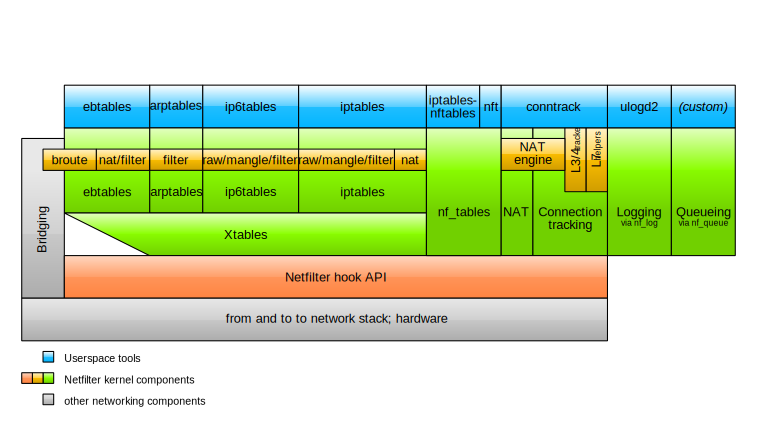
\includegraphics[width=\linewidth]{images/nf-components.eps}
    \caption[Componenti di Netfilter]{Componenti di Netfilter:\footnotemark}
    \label{fig:netfilter}
\end{figure}
\noindent Dalla figura \ref{fig:netfilter} risulta evidente la maggiore complessità e
\footnotetext{\href{http://inai.de/images/nf-components.svg}{Sorgente} (CC BY-SA 3.0).}%
ridondanza di Xtables rispetto a nftables. L'unica area verde dedicata a
nf\_tables rappresenta il codice del kernel mentre le componenti userspace
sono l'utilità nft e il tool di retrocompatibilità iptable-nftables per poter
inserire regole con la vecchia sintassi.

Nftables riduce il numero di linee di codice nel kernel riorganizzando e
unificando quello che in iptables è replicato quattro volte per i diversi protocolli.
Inoltre nftables introduce strutture dati (insiemi\footnote{Iptables non
    gestisce nativamente gli insiemi ma esiste il tool ipset che fornisce a
iptables questa funzionalità.}, dizionari, mappe e concatenazioni) che permettono di
semplificare e ottimizzare le regole del firewall. Contestualmente migliorano la
leggibilità delle regole e le prestazioni.

Iptables prevede che ogni regola viene introdotta da un comando *tables con
relativi argomenti; nftables invece offre un proprio linguaggio col quale
viene descritto e configurato l'intero firewall e le regole vengono attivate
atomicamente. Anche questo migliora la leggibilit\`a e la gestione nel tempo
degli insiemi di regole.

\section{Nftables successore di iptables?}

Nei casi precedenti all'uscita di un nuovo framework (ipfwadm, ipchains, iptables)
la migrazione si rendeva necessaria anche perché il vecchio veniva dichiarato obsoleto
e non più supportato.
Questo non è ancora accaduto con nftables e tutto fa pensare che in questo
caso il percorso sarà diverso; vedremo in seguito come si possa
prospettare la transizione da iptables al suo successore.

\chapter{Firewall Linux nella rete Galliera}

\section{Cenni storici}

Come anticipato nell'introduzione, la LAN dell'ospedale Galliera è collegata
ad internet dal 1996 e da sempre tutti i principali servizi di rete sono stati
gestiti da macchine Linux delle quali mi sono personalemente occupato.
Non fanno eccezione i servizi di firewall (filtering e NAT) che nel 1996
furono realizzati con ipfwadm.

L'uso del firewall nei primi anni era limitato all'implementazione di filtri
per il traffico in ingresso verso i servizi esposti a internet e al {\em
masquerading} (SNAT) degli indirizzi IPv4 interni (di classe riservata).

Ad ogni evoluzione dei sistemi di firewall di Linux abbiamo provveduto ad
aggiornare i sistemi convertendo di volta in volta le regole e approfittando
delle nuove funzionalità introdotte.

\section{Architettura attuale}
Nel tempo è cresciuto il numero di sottoreti collegate, di servizi esposti e
di conseguenza la complessità delle regole configurate.

La situazione attuale consiste di due firewall iptables, uno esterno ed uno
interno.  Il firewall esterno regola il traffico tra internet, DMZ e reti
locali; quello interno disciplina il traffico tra le reti locali e l'esterno.
\begin{figure}[H]
\begin{center}
    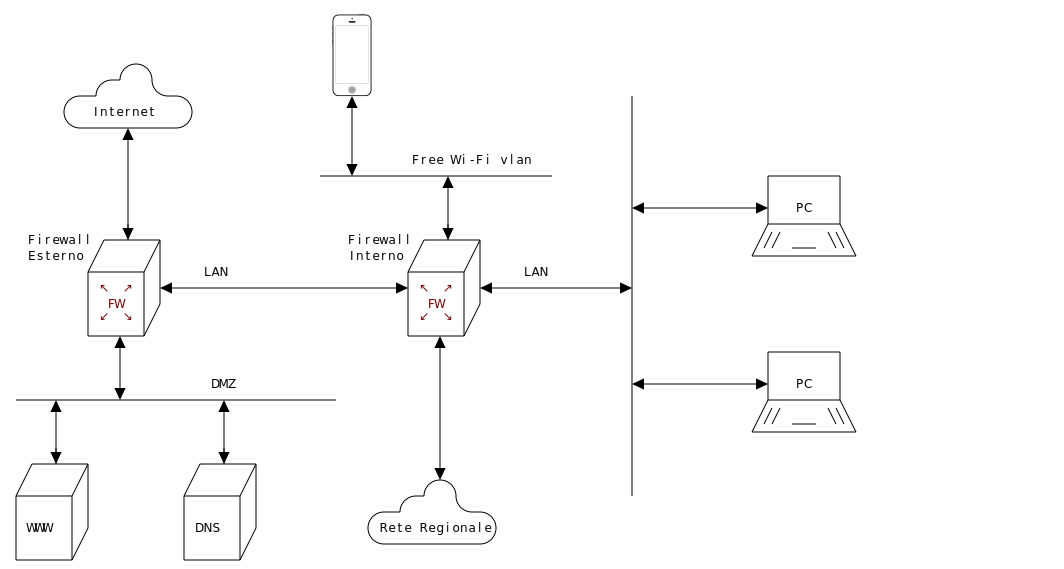
\includegraphics[width=\linewidth]{images/net.eps}
    \caption{Schema delle reti e dei due firewall}
    \label{fig:rete}
\end{center}
\end{figure}
\noindent Il firewall esterno \`e anche il terminatore delle connessioni VPN (IPsec,
OpenVPN e WireGuard) e implementa una serie di regole ``blacklist'' i cui
indirizzi provengono da:
\begin{itemize}
    \item \href{https://iplists.firehol.org/?ipset=firehol\_level1}{''FireHol
        Level1''}\footnote{\url{https://iplists.firehol.org/?ipset=firehol\_level1}} (oltre
    7000 sottoreti),
    \item \href{https://ransomwaretracker.abuse.ch/downloads/RW\_IPBL.txt}{''Ransomware
        Tracker''}\footnote{\url{https://ransomwaretracker.abuse.ch/downloads/RW\_IPBL.txt}}
    (circa 400 indirizzi)
    \item fail2ban su ssh: blacklist auto-generata in base ai tentativi
    falliti di connessione via ssh (circa 9000 indirizzi al momemnto)
    \item lista di indirizzi di botnet autoprodotta da script che analizzano
    tentativi di bruteforce tipicamente su servizi di posta (oltre 12.000
    indirizzi)
\end{itemize}
Il totale delle regole supera le 20 mila.

Il firewall interno invece gestisce le regole del captive portal: si tratta di
abilitare il traffico verso internet dei dispositivi wireless di coloro che si
sono registrati tramite interfaccia web.
Il sistema di registrazione e abilitazione, che ho realizzato con la
collaborazione di un collega, agisce classificando i pacchetti in base al mac
address: i pacchetti con mac adddress abilitato vengono inoltrati
regolarmente, i rimanenti vengono marcati\footnote{L'associazione del ``mark''
al pacchetto è realizzata all'interno del kernel, il pacchetto resta
inalterato.} e deviati verso la pagina web che propone la registrazione.

Registriamo 80/90 nuovi dispositivi al giorno e sono 100.000 quelli
che hanno usufruito del servizio a partire dal 2012.  Non avendo specificato
termini di scadenza la lista di mac address non decresce mai; ad esempio al
momento sono presenti oltre 23 mila indirizzi ethernet.  Di tanto in tanto si
eseguono interventi di cancellazione delle autorizzazioni pi\`u vecchie.

\section{Problemi dell'infrastruttura}

Nella sezione precedente ho messo in evidenza le dimensioni degli insiemi di
indirizzi perché, durante il 2017, proprio la gestione di tante regole ha 
portato alla luce alcune carenze della soluzione implementata.

Per ogni indirizzo era prevista una regola\footnote{Di tipo {\em
REJECT} per le blacklist e di tipo {\em RETURN} per la gestione della rete wifi
free.}, cosa che comportava scorrere una lista di (decine di) migliaia di
regole per poter classificare un pacchetto.

Questo approccio non è efficiente in quanto il lavoro del firewall cresce
linearmente col numero di regole e il throughput ne risente.
Tipicamente la soluzione in questi casi consiste nell'usare una struttura dati
di tipo hash.
Iptables non prevede strutture dati di questo tipo; esiste per\`o uno
strumento esterno, ipset, che lo supporta in questa funzionalità permettendo di
ridurre decine di migliaia di regole ad un unica regola (nello specifico una
regola per ogni insieme).

I problemi dovuti all'eccessivo numero di regole sono stati quindi risolti
usando ipset su entrambe i firewall\footnote{L'introduzione dei set ha
richiesto la revisione del codice del captive portal e dei programmi di
generazione di blacklist.}.

\section{Opportunità di migrazione a nftables}

L'uso dei set di indirizzi ha risolto i problemi, tuttavia ho voluto
verificare cosa comportasse la migrazione da iptables a nftables; in termini
di impegno necessario rispetto ai vantaggi offerti.

Nftables si propone come framework completamente nuovo, più che come
evoluzione di iptables, l'interfaccia di configurazione è diventata simile ad
un linguaggio di programmazione e la struttura di tabelle e catene non
\`e pi\`u vincolata dal framework. Ci\`o significa dover riprogrammare tutte le
logiche all'interno del nuovo framwork. Anche se esistono i tool di traduzione
di regole, parte del lavoro va eseguita manualmente.

\chapter{Nftables}

Nel seguito utilizzeremo la convenzione per cui righe come le seguenti
rappresentano uno script di configurazione di nftables:
\begin{lstlisting}[style=customc]
table ip filter {
        chain input {type filter hook input priority 0; policy drop; 
        	ip saddr 42.0.0.0/ accept;
	}
}
\end{lstlisting}

Queste invece rappresentano comandi, eseguiti da linea di comando da root, con
relativo output:
\begin{lstlisting}
# nft list ruleset | grep -w "comment.*DEBUG"
ip saddr @testsources nftrace set 1 comment "DEBUG: XXX remove in production"
\end{lstlisting}

\section{Caratteristiche di nftables}
Vediamo quali sono le principali novit\`a introdotte da nftables.
\begin{itemize}
    \item supporto nativo per dual stack IPv4 e IPv6
    \item supporto nativo per strutture dati (importanti per le prestazioni):
    insiemi, mappe, dizionari e concatenazioni
    \item interessanti strumenti di debug e tracing
    \item aggiunta dell'hook ingress per migliorare le prestazioni
    \item layout di regole flessibile, partendo da un insieme vuoto, rispetto
    al classico layout statico di iptables (filter/INPUT, nat/PREROUTING,
    \ldots)
    \item contatori opzionali e azioni multiple in una singola regola (ad
        esempio si pu\`o incrementare un contatore, scrivere nel log e eseguire NAT nella
    stessa regola)
    \item migliori opzioni di gestione dell'insieme di regole, aggiornamenti
    delle regole completamente atomici e incrementali
\end{itemize}
Si possono quindi inserire regole che valgono contestualemnte sia per IPv4 che
per IPv6,
mentre le strutture dati consentono di migliorare le prestazioni e la
leggibilit\`a delle regole, oltre a non richiedere il supporto di tool
esterni.

Sono previsti utili strumenti di log e debug: ad esempio \`e possibile
tracciare l'intero percorso di un singolo pacchetto attraverso le regole e la
funzione di monitor permette di osservare in tempo reale le modifiche alle
regole di firewall.  Molto utile per la gestione è inoltre la possibilità di
introdurre commenti associati alle regole: chiedendo al kernel di elencare le
regole attive appaiono anche i relativi commenti; ci\`o \`e diverso dall'avere
il commento nel codice sorgente che nel frattempo potrebbe essere stato
modificato o addirittura perso.

Vediamo un semplice esempio: vogliamo verificare se qualcuna tra le regole
attualmente caricate ha nel commento la stringa ``DEBUG'':
\begin{lstlisting}
# nft list ruleset | grep -w "comment.*DEBUG"
ip saddr @testsources nftrace set 1 comment "DEBUG: XXX remove in production"
\end{lstlisting}

\section{Packet flow in nftables}

\begin{figure}[H]
    \centering
    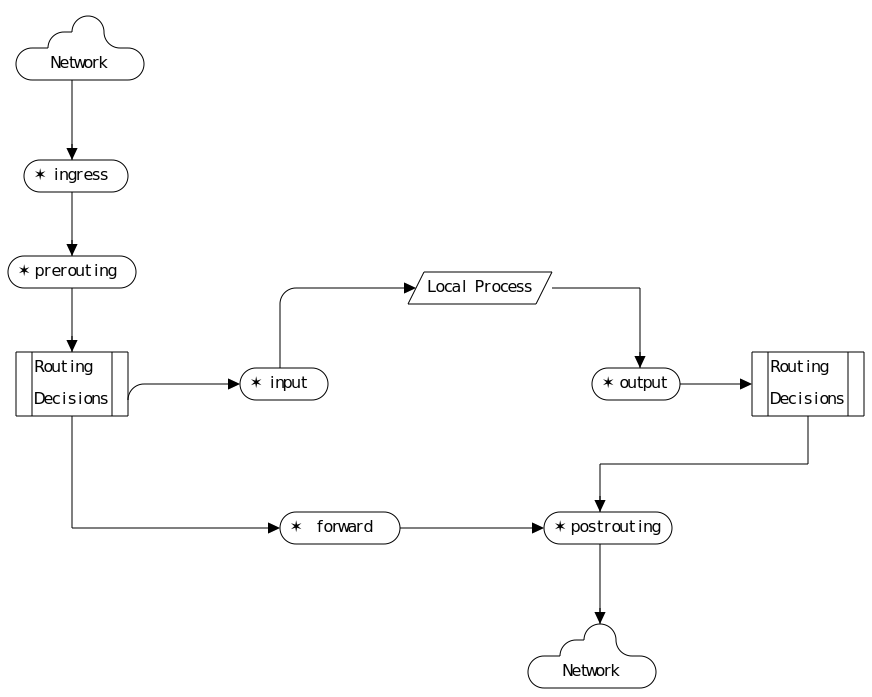
\includegraphics[width=\linewidth]{images/flow.eps}
    \caption{Schema del flusso di pacchetti in nftables}
    \label{fig:flow}
\end{figure}
Le regole vengono organizzate in catene che a loro volta sono contenute in
tavole. Le tavole sono associate ad una delle famiglia che determina il tipo
di traffico visibile nella tavola. Le famiglie sono: ip (per il traffico
IPv4), ip6 (per IPv6),
inet (sia IPv4 che IPv6), arp, bridge e netdev (vede tutto il traffico).

Lo schema \ref{fig:flow} rappresenta i possibili percorsi di un pacchetto e
l'asterisco evidenzia gli hook ai quali si possono associare le catene:
\begin{itemize}
    \item ingress
    \item prerouting
    \item input
    \item output
    \item forwarding
    \item output
    \item postrouting
\end{itemize}
La possibilit\`a di intervenire precocemente sul pacchetto, appena il driver
dell scheda di rete lo passa al livello superiore, \`e utile per gestire
attacchi tipo DDoS o per limitare la banda senza appesantire il lavoro del
kernel: questo \`e reso possibile dall'hook ingress che interviene prima del
prerouting.
Catene associate all'hook ingress sono definite in tavole della
famiglia netdev. Scartare i pacchetti a questo livello \`e due volte
pi\`u efficiente rispetto al drop in prerouting.

I pacchetti che sono destinati a qualche processo locale (cioè sono indirizzati
all'host stesso) sono gestiti tramite l'hook input ed analogamente quelli
generati da processi locali tramite l'hook output.

Il traffico che deve essere inoltrato fra le due reti viene gestito tramite
l'hook forward.

Il NAT interviene in prerouting (DNAT) e postrouting (SNAT).

Il layout iniziale di nftables \`e semplicemente l'insieme vuoto;
l'amministratore \`e libero di configurare tavole (table) e catene
(chain)\footnote{Le tavole sono contenitori di catene che a loro volta
contengono regole.} nel modo pi\`u adatto al problema da risolvere.

In iptables i contatori dei pacchetti, transitati da ogni catena, non si
possono disabilitare; con nftables si pu\`o e sono disabilitati per default:
attivandoli solo quando necessario possono migliorare le prestazioni.

Poter indicare pi\`u azioni per una singola regola rende pi\`u leggibile e
consistente il codice; con iptables spesso è necessario saltare ad un'altra
catena contenente le diverse azioni. Ad esempio, vediamo due soluzioni
iptables per scartare un pacchetto registrando l'operazione
nei log: 

\begin{lstlisting}
# iptables -t filter -A OUTPUT -d 10.0.0.1 -j LOG # Log, continue to next rule
# iptables -t filter -A OUTPUT -d 10.0.0.1 -j DROP # Drops the same packet
\end{lstlisting}
oppure 
\begin{lstlisting}
# iptables -t filter -N LOGGING # Create non-base chain for logging
# iptables -t filter -A LOGGING -j LOG # Add rule to logging chain to LOG
# iptables -t filter -A LOGGING -j DROP # Add rule to logging chain to DROP
# iptables -t filter -A OUTPUT -d 10.0.0.1 -j LOGGING # Jump LOGGING if match
\end{lstlisting}
con nftables \`e sufficiente una sola regola:
\begin{lstlisting}
# nft add rule ip filter output ip daddr 10.0.0.1 log drop
\end{lstlisting}
Un esempio minimale di configurazione per un server web pu\`o essere
il seguente:
\lstinputlisting[caption=Semplice esempio per server web, style=customc]{nftables-web.conf}
Notare, riga 9, che le connessioni già stabilite o relative a
connessioni già stabilite, informazione ricavata dalla conntrack table,
sono accettate.
I servizi aperti all'esterno sono ssh, http e https, tutto il resto
viene scartato (drop) senza l'invio "ICMP host unreachable". Inoltre i
pacchetti rifiutati vengono contati (counter).

\lstinputlisting[caption=Semplice esempio di router/firewall, style=customc]{nft-simple-forward.nft}
Questo esempio descrive il comportamento di un semplice
router/firewall. La tavola è associata ai protocolli IPv4 e IPv6 (inet) e
definisce due insiemi di indirizzi (righe 2 e 7).
Al solito viene accettato traffico relativo a connessioni attive (riga 13)
mentre viene scartato il traffico non valido (causato da stealth port scan, da
problemi nella conntrack table o da anomalie benigne).
Oltre ad accettare connessioni verso qualsiasi server ssh e http(s), un
verdetto positivo è previsto anche per qualsiasi connessione verso i server
elencati ei due insiemi my\_ipv4\_addrs e my\_ipv6\_addrs.
Per ognuna delle categorie sopra elencate viene attivato il contatore.

\section{Strumenti di debug e tracing}
Ritengo che il sistema di tracing offerto da nftables sia di ottima qualit\`a;
\`e fondamentale per la rapida individuazione dei bug durante la
sperimentazione e lo sviluppo dei ruleset.
Il tracing viene attivato impostando una metainformazione relativa al pacchetto: nftrace=1.
\begin{lstlisting}
# nft add rule filter forward udp dport 53 meta nftrace set 1
\end{lstlisting}
Dal momento che transita dalla catena di forward, ogni pacchetto destinato ad un DNS server riporter\`a
i dettagli del suo percorso attraverso l'insieme di regole.

Per osservare il resoconto del ``viaggio'' del pacchetto \`e necessario attivare il
monitor da console: i pacchetti con nftrace settato invieranno al monitor le informazioni
con i dettagli relativi al percorso seguito.
Questo ad esempio \`e il percorso di un pacchetto destinato ad un DNS server:
\begin{lstlisting}
# nft monitor
trace id e7d627c0 ip captive forward packet: iif "eth1" oif "eth0" ether saddr 00:16:3e:05:12:55 ether daddr 00:16:3e:35:e7:80 ip saddr 193.168.100.159 ip daddr 8.8.8.8 ip dscp cs0 ip ecn not-ect ip ttl 63 ip id 36018 ip length 59 udp sport 40220 udp dport domain udp length 39 @th,64,96 49749720051147984142130479104
trace id e7d627c0 ip captive forward rule udp dport domain nftrace set 1 (verdict continue)
trace id e7d627c0 ip captive forward verdict continue
trace id e7d627c0 ip captive forward
trace id e7d627c0 ip captive nat_postrouting verdict continue
trace id e7d627c0 ip captive nat_postrouting
\end{lstlisting}

\chapter{Migrazione del Captive Portal}

%Il progetto che sto realizzando prevede molte attivit\`a, ad esempio gli
%automatismi di gestione delle regole tramite l'uso di git e Ansible.

Per captive cortal si intende una configurazione della rete in cui il
dispositivo che si collega la prima volta viene reindirizzato ad una pagina web
tramite la quale si identifica ottenendo l'autorizzazione all'uso della rete.

Nel nostro caso l'identificazione avviene fornendo il numero di cellulare al
quale viene inviato un codice via SMS. L'utente restituisce questo codice
attraverso la stessa pagina del captive portal e cos\`i facendo il dispositivo
viene autorizzato: il mac address viene aggiunto dinamicamente tra quelli
che il firewall non deve bloccare.

Lo schema di verifica e autorizzazione del traffico è il seguente:
\begin{enumerate}
    \item il pacchetto viene analizzato per verificare se il mac
    address è stato autorizzato
    \begin{itemize}
        \item sì: allora finisce l'analisi e il pacchetto viene inoltrato
        \item no: il pacchetto viene marcato (0x63)
    \end{itemize}
    \item in fase di prerouting, se il pacchetto è marcato ed la porta di
    destinazione è http allora viene reindirzzato (DNAT) alla pagina del
    captive portal
    \item negli altri casi (pacchetto marcato e traffico non http) allora il
    pacchetto viene scartato in fase di forwarding
\end{enumerate}

\section{Captive Portal con iptables}
\label{lab:captive}
La configurazione di iptables che realizza quanto descritto sopra è la
seguente:
\lstinputlisting[caption=Mangle per wifi free, style=customc,
label={lst:iptables-wifi}]{captive-iptables.conf}
Il listato \ref{lst:iptables-wifi} rappresenta la configurazione del
firewall limitatamente alle regole strettamente necessarie a realizzare la
funzionalità di captive portal. Il fatto di aver eliminato le regole non
pertinenti il caso in esame può far sembrare inutili o ridondanti alcune di
quelle elencate.

Le prime nove righe sono relative alla marcatura in fase di prerouting:
\begin{itemize}[itemindent=2em]
    \item[(riga 4)] il traffico proveniente dalla rete wifi (192.168.16.0/20)
    verrà analizzato dalla catena internet (salta alla riga 8)
    \item[(riga 8)] se il mac address sorgente è contenuto nel set captive\_ok
    ritorna
    \item[(riga 9)] marca il pacchetto con il valore 0x63 (99 decimale)
  \end{itemize}
  La tavola filter, riga 11:
  \begin{itemize}[itemindent=2em]
    \item[(riga 12)] di default scarta i pacchetti che non soddisfano una delle regole
    \item[(riga 13)] accetta il traffico relativo a connessioni già attivo
    \item[(riga 14)] scarta i pacchetti marcati con il valore 0x63
\end{itemize}
La tavola di NAT ha il compito di indirizzare il traffico http verso il sito
del captive portal.
Le righe dalla $20$ in poi sono relative all'insieme captive\_ok, quello che contiene i mac
address autorizzati\footnote{Qui abbiamo usato indirizzi fittizi.}
L'intestazione indica che si tratta di un insieme di mac address e a
seguire sono elencati gli elementi dell'insieme.

\section{Captive Portal nella versione nftables}
Un'implementazione della logica del captive portal in nftables è la seguente:
\lstinputlisting[caption=Captive portal con nftables, style=customc,
label={lst:nftables-wifi}]{captive-nftables.conf}
Possiamo intanto notare due cose:
\begin{itemize}
	\item il linguaggio prevede la definizione di variabili
	
	\item le due catene, filter\_prerouting e nat\_prerouting, sono di tipo diverso
	(una filtra e l'altra esegue il NAT) ma sono agganciate allo stesso hook
    (prerouting): la priorità definisce quale deve essere l'ordine di consultazione
\end{itemize}
L'attivazione di un dispositivo si effettua inserendone il mac address nell'insieme
captive\_ok:
\begin{lstlisting}
# nft add element captive captive_ok {00:16:3e:05:12:55}
\end{lstlisting}
Passiamo ora a descrivere alcune funzionalità specifiche di nftables.

\section{Autorizzazioni temporizzate}

Vogliamo che
l'autorizzazione all'uso della rete wifi scada dopo 15 giorni.  Per fare ciò
dobbiamo modificare la definizione del set, alla riga 5 del listato
\ref{lst:nftables-wifi}, introducendo un timeout\footnote{Durante la
    sperimentazione ho identificato un bug che al
    momento risulta ancora aperto. Non si riescono ad impostare timeout >
24d20h31m23s.\\Vedi \url{https://bugzilla.netfilter.org/show\_bug.cgi?id=1237}
} in questo modo:
\begin{lstlisting}[style=customc, firstnumber=5]
set captive_ok { type ether_addr; timeout 15d; }
\end{lstlisting}
Ogni elemento inserito nell'insieme verrà eliminato automaticamente dopo 15
giorni. \`E possibile verificare in ogni istante quanto tempo resta prima
della scadenza:
\begin{lstlisting}
# nft add set captive captive_ok_timeout { type ether_addr\; timeout 15d\; }
# nft list set captive captive_ok_timeout
table ip captive {
        set captive_ok_timeout {
                type ether_addr
                timeout 15d
        }
}
# nft add element captive captive_ok_timeout {6c:0b:84:91:7d:a4}
# sleep 5 && nft list set captive captive_ok_timeout
table ip captive {
        set captive_ok_timeout {
                type ether_addr
                timeout 15d
                elements = { 6c:0b:84:91:7d:a4 expires 14d23h59m54s }
        }
}
\end{lstlisting}
Verifichiamo che ogni elemento disponga di un proprio timer indipendente:
\begin{lstlisting}
# nft add element captive captive_ok_timeout {02:0a:76:09:41:8b}
# nft list set captive captive_ok_timeout
table ip captive {
        set captive_ok_timeout {
                type ether_addr
                timeout 15d
                elements = { 02:0a:76:09:41:8b expires 14d23h59m57s,
                             6c:0b:84:91:7d:a4 expires 14d23h56m4s }
        }
}
\end{lstlisting}
\newpage
\noindent Alternativamente o in aggiunta al timeout di default, è possibile definire un
set in cui ogni elemento può essere esplicitamente dichiarato con il proprio
timeout:

\begin{lstlisting}
# nft add set captive captive_ok_timeout_flag { type ether_addr\; flags timeout\; timeout 15d\; }
# nft add element captive captive_ok_timeout_flag {02:0a:76:09:41:8b}
# nft list set captive captive_ok_timeout_flag
table ip captive {
        set captive_ok_timeout_flag {
                type ether_addr
                timeout 15d
                elements = { 02:0a:76:09:41:8b expires 14d23h59m57s }
        }
}
# nft add element captive captive_ok_timeout_flag {02:0a:88:01:c3:51 timeout 42m}
# nft list set captive captive_ok_timeout_flag
table ip captive {
        set captive_ok_timeout_flag {
                type ether_addr
                timeout 15d
                elements = { 02:0a:76:09:41:8b expires 14d23h58m51s,
                             02:0a:88:01:c3:51 timeout 42m expires 41m58s }
        }
}
\end{lstlisting}
La scadenza automatica degli elementi degli insiemi semplifica la gestione del sistema in quanto non è necessario intervenire con altri
strumenti per eliminare i mac address scaduti.

\section{Aggiornamento del timeout}
In realt\`a sarebbe auspicabile un comportamento pi\`u {\em intelligente}: se un utente \`e 
un ospite frequente\footnote{Ad esempio perch\'e dipendente.} vorremmo evitare
di dovergli chiedere la registrazione ogni 15 giorni;
vogliamo invece far scadere l'autorizzazione 15 giorni dopo l'ultimo utilizzo del servizio.
Per ottenere ci\`o \`e necessario aggiornare il timeout
ogni volta che si osserva transitare un pacchetto generato dal singolo client.

Nftables \`e in grado di aggiornare dinamicamente i set in funzione del
percorso del pacchetto: proprio la funzionalit\`a che ci serve.
Apportiamo quindi questa modifica allo script \ref{lst:nftables-wifi}:

\begin{lstlisting}[style=customc,firstnumber=6]
chain filter_prerouting {
    type filter hook prerouting priority 0; policy accept;
    ip saddr $WIFINET ether saddr @captive_ok set update ether saddr timeout 15d @captive_ok return
    ip saddr $WIFINET mark set 0x63
}
\end{lstlisting}
La riga numero 8 del listato \ref{lst:nftables-wifi} adesso non solo ritorna,
di fatto autorizzando il pacchetto, ma contestualmente aggiorna l'elemento
reimpostandone la validit\`a a 15 giorni.

Realizzare applicativamente questa funzionalit\`a avrebbe significato
doversi confrontare con almeno tre domini diversi: le regole del firewall, il
database delle autorizzazioni e i log. Una soluzione affidabile non sarebbe stata di
facile realizzazione.

\section{Limitazione della banda}

Potrebbe essere necessario in certi casi imporre qualche limite alla banda
dedicata agli utenti della rete wifi. Anche in questo caso nftables offre una
soluzione che risulta semplice da implementare
nel linguaggio di definizione delle regole.

Il caso pi\`u semplice consiste nel limitare la banda occupata globalmente
dalla rete wifi.
Facendo sempre riferimento allo script \ref{lst:nftables-wifi}, riscriviamo
la catena di forward in questo modo:

\begin{lstlisting}[style=customc,firstnumber=18]
chain forward {
    type filter hook forward priority 0; policy accept;
    limit rate over 8 mbytes/second drop
    ct state established,related accept
    mark 0x63 drop
}
\end{lstlisting}
Avendo introdotto la riga 20 imponiamo che il traffico inoltrato non possa
superare 8 mbytes, i pacchetti in eccesso vengono scartati.
Questa operazione risulta per\`o  pi\`u efficiente\footnote{Vedi ad esempio
\url{https://netdevconf.org/1.2/slides/oct6/08\_nftables\_Load\_Balancing\_with\_nftables\_II\_Slides.pdf}}
se eseguita in ingress.
In effetti nella configurazione delle regole per il captive portal ho scelto questo
approccio.
\begin{lstlisting}[style=customc,firstnumber=18]
table netdev wifirate {
    chain download {
        # interfaccia verso internet
        type filter hook ingress device eth2 priority 0;
        limit rate over 8 mbytes/second counter drop
    }
    chain upload {
        # interfaccia verso wifi
        type filter hook ingress device eth1 priority 0;
        limit rate over 8 mbytes/second counter drop
    }
}
\end{lstlisting}
La tabella wifirate limita la banda entrante dall'interfaccia eth2, download da internet,
e la banda entrante dall'interfaccia eth1, cio\`e l'upload verso internet.

\noindent Quella che segue \`e una variante che garantisce che la limitazione si applichi solo alla rete wifi e che
permette di oltrepassare il limite per brevi periodi se necessario (burst):
\begin{lstlisting}[style=customc,firstnumber=20]
ip daddr $WIFINET limit rate over 6 mbytes/second burst 10 mbytes/second drop
\end{lstlisting}
Una regola ancora pi\`u raffinata \`e la seguente. Qui sfruttiamo i meter e la concatenazione:
\begin{lstlisting}[style=customc,firstnumber=20]
ip daddr $WIFINET meter rate-meter { ip saddr . ip daddr limit rate over 3 mbytes/second burst 5 mbytes/second } drop
\end{lstlisting}
L'operatore ``.'' concatena i due indirizzi, sorgente e destinazione, generando la chiave
dell'elemento al quale si applica il limite di 3 megabyte al secondo.

Queste sono solo alcune delle potenziali\`a di nftables, ma sono quelle che
risultano pi\`u interessanti per i nostri scopi.

\chapter{Strumenti di sviluppo e test}


\section{Virtualizzazione}

Per realizzare i test delle regole in un ambiente simulato, ho configurato tre
server virtuali libvirt+lxc, cio\`e sostanzialmente tre Linux container con
sistema operativo Debian 9.4 (sia per i guest che per l'host); l'hardware
consiste di un laptop Intel i5 dual core.

Una delle tre macchine, chiamata fw, simula il firewall tra una LAN e una rete
pubblica. La seconda macchina, chiamata pc, rappresenta un client all'interno
di una rete locale mentre la terza simula un server in internet, chiamato
wikipedia.

Lo strato di virtualizzazione della rete \`e quello offerto da libvirt; sono
state definite le reti loc e net rispettivamente per la LAN e per internet.
\begin{figure}[H]
\begin{center}
      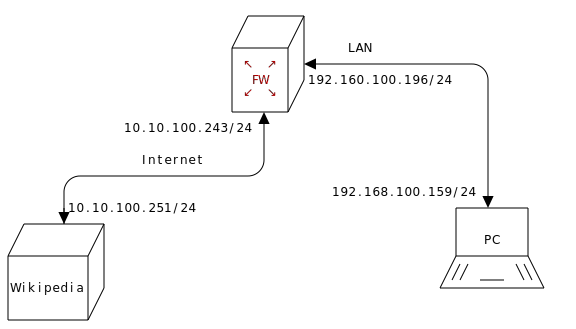
\includegraphics[width=.7\linewidth]{images/vnet.eps}
      \caption{Macchine virtuali}
      \label{fig:vnet}
\end{center}
\end{figure}
\noindent In questa configurazione le prestazioni della rete sono state valutate con
iperf(1) e wget(1).
Nel primo test, routing, la macchina fw agisce come semplice router.
Nel test mark \`e attiva la verifica dell'appartenenza del mac address
all'insieme degli indirizzi autorizzati ma l'insieme \`e costituito da un solo
elemento.
Nel test mark-full l'insieme \`e costituito da 23.000 elementi.
Il risultato sembra confermare che nftables pu\`o gestire
insiemi grandi dimensioni senza eccessive difficolt\`a\footnote{Ovviamente non
possiamo attribuire un valore assoluto al test. Quello che ci interessa
evidenziare \`e che che non si ravvisano differenze sostanziali nei tre casi.}.

\begin{center}
  \label{tab:benchmark}
  \begin{table}[ht]
    \centering % used for centering table
     \begin{tabular}{@{}llcc@{}}
     \toprule
     {\bf Configurazione} & {\bf iperf} & {\bf wget 4GB} \\ \midrule
         routing  & 32.6                & 4.5 \\
         mark     & 30.3                & 4.4 \\ 
         mark-full& 30.2                & 4.4 \\ \bottomrule
      \end{tabular}  
    \caption{Benchmark} % title of Table
  \end{table}
\end{center}


\section{Debug}

Il debug come accennato in precedenza \`e stato facilitato dal sistema di
packet tracing.
Ovviamente sono stati fondamentali anche i tool tradizionali, uno su tutti tcpdump.

Volendo scendere a livello pi\`u basso si pu\`o arrivare a verificare il
bytecode iniettato nel kernel quando si inserisce una regola:
\begin{lstlisting}[style=customc]
# nft --debug=netlink add rule atable arule ip saddr 10.0.0.0/8 accept            
ip atable arule
  [ payload load 4b @ network header + 12 => reg 1 ]
  [ bitwise reg 1 = (reg=1 & 0x000000ff ) ^ 0x00000000 ]
  [ cmp eq reg 1 0x0000000a ]
  [ immediate reg 0 accept ]
\end{lstlisting}
Il payload \`e il pacchetto in esame.
\begin{itemize}
    \item alla riga 3 vengono caricati nel registro numero 1, 4 byte a partire dalla dodicesima posizione dell'header del
pacchetto: cio\`e l'indirizzo IPv4 sorgente
    \item alla riga 4 viene applicata la netmask per caricare nel registro 1
        il byte pi\`u significativo dell-indirizzo
    \item alla riga 5 il registro 1 viene confrontato con il valore 0xa (10 decimale)
\end{itemize}
se il confronto ha successo il pacchetto viene accettato.

\chapter{Considerazioni finali}

Nonostante gli indiscutibili vantaggi di nftables rispetto ad iptables, non
sembra che la sostituzione possa avvenire a breve.  La difficolt\`a di
nftables nello scalzare iptables dipende dal fatto che iptables nei sui 17/18
anni di vita si \`e diffuso molto (datacenter, virtualizzazione, container,
\ldots) ed ha arricchito le sue funzionalit\`a, magari in modo non elegante ma
comunque efficace. Per certi versi la situazione assomiglia a quella tra IPv4
e IPv6.

Paradigmatica a questo proposito \`e la decisione presa da WikiMedia Foundation
dopo aver discusso sull'argomento {\em netfilter software at WMF: iptables vs
nftables}\footnote{\url{https://phabricator.wikimedia.org/T187994}}.  La
proposta di migrare l'infrastruttura di WMF \`e stata avanzata da Arturo
Borrero, mantainer del pacchetto nftables per Debian e operator del ``cloud
team'' di Wikimedia. Lui stesso, dopo aver previsto che la migrazione completa
richiederebbe 1 se non 2 anni, conclude che non \`e il momento:
\begin{quote}
    {\em EOF. I propose we follow up in the future.}
\end{quote}

\noindent Come nel caso di WikiMedia per molti il ragionamento sembra essere lo stesso:
{\em``tutto sta
funzionando con iptables, non si evidenziano problemi, lo sforzo per passare a
    nftables \`e importante: non conviene.''}.

\section{eBPF}

Quello che invece sembra rappresentare il futuro \`e eBPF:
enanched Berkeley Packet Filtering\footnote{eBPF fa molto di pi\`u che filtrare
pacchetti: \`e anche in grado di fare raw tracing in modo simile a quello di
DTrace e SystemTap.\\Un buon punto di partenza \`e
\url{https://github.com/iovisor/bcc}}.
L'articolo su Linux Weekly News del 19 febbraio 2018
\footnote{\url{https://lwn.net/Articles/747551/}} dal titolo ``BPF comes to firewalls''
dice tra l'altro:

\begin{quote}
    {\em \ldots Miller\footnote{Si tratta di David Miller, uno dei mantainer dello stack
TCPI/IP di Linux} said in the discussion that nftables failed to address the
performance problems in Linux's packet-filtering implementation, driving users
toward user-space networking technologies instead. There is a real possibility
that nftables could end up being one of those experiments that is able to shed
some light on the problem space but never takes over in the real world.}
\end{quote}


\section{eBPF/XDP}
Quando abbiamo visto i possibili utilizzi dell'hook ingress consideravamo
un vantaggio in termini di prestazioni il fatto di essere ``pi\`u vicini'' al
driver della scheda di rete. XDP (eXpress Data Path) si spinge oltre
demandando (offloading) il filtraggio, e altro, direttamente al firmware della scheda di
rete (vedi \url{https://www.iovisor.org/technology/xdp}).

Vengono gi\`a prodotte e commercializzate le cosiddette SmartNIC\footnote{Ad esempio
    \url{https://www.netronome.com/products/smartnic/overview/}},
    schede di rete progettate appositamente per l'offloading.
    
    Qualcuno
    non vede di buon occhio questo approccio perch\'e teme si possa trattare di tentativi di
    ``kernel
    bypass'' ma gli sviluppatori di soluzioni eBPF/XDP forniscono
    rassicurazioni in questo senso\footnote{\url{https://www.netronome.com/blog/avoid-kernel-bypass-in-your-network-infrastructure/}}.

\section{Conclusioni}

Nonostante il fermento intorno alle nuove soluzioni di packet filtering \`e
indubbio che iptables non verr\`a abbandonato nel breve periodo.  Le ricadute pratiche
del lavoro di sperimentazione svolto si limiteranno all'introduzione di
nftables sul firewall interno in virt\`u delle funzionalit\`a di
cui abbiamo discusso nella sezione \ref{lab:captive}; non ritengo utile
portare avanti la migrazione del firewall esterno.
